%!TEX root = 多体系统动力学.tex
\chapter{系统树形拓扑描述}
\begin{figure}[htbp]
    \centering
    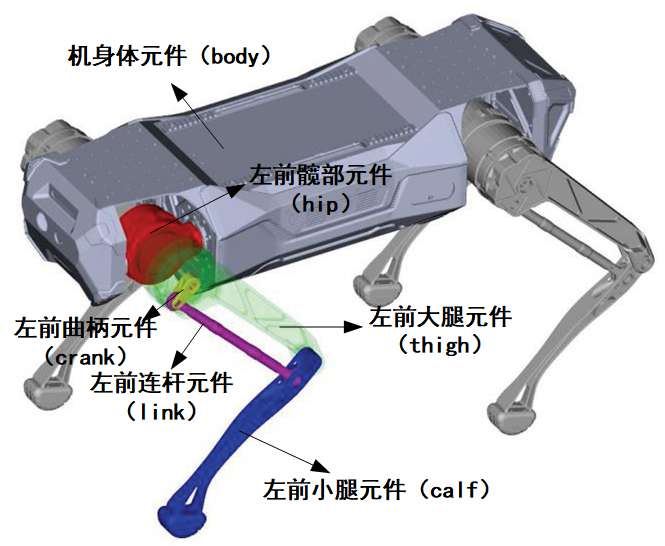
\includegraphics[width=0.5\textwidth]{figures/四足机器人动力学模型.PNG}
    \caption{四足机器人动力学模型}
    \label{fig:四足机器人动力学模型}
\end{figure}
略去几何尺寸信息，只保留相邻体之间的连接关系，即可得到四足机器人的树形拓扑描述。如下图：
\begin{figure}[htbp]
    \centering
    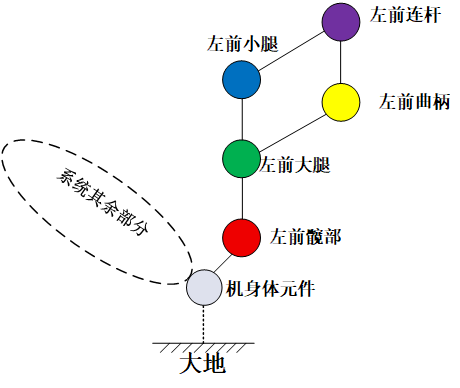
\includegraphics[width=0.5\textwidth]{figures/四足机器人动力学模型拓扑图.png}
    \caption{四足机器人动力学模型拓扑图}
    \label{fig:四足机器人动力学模型拓扑图}
\end{figure}

若按照实际接触情况，即将四足机器人与地面接触的腿视为根节点，则与地面会有四个虚铰，不便于后续的树形化处理。为了便于树形化处理，我们将四足机器人与地面接触的腿视为叶节点，四足机器人身体元件视为根节点，同时将小腿与地面之间认为存在刚度与阻尼进行处理。
